\documentclass{article}
\usepackage{hyperref}
\usepackage{cite}
\usepackage{listings}
\usepackage{graphicx}
\graphicspath{ {latex_images/} }

\begin{document}
\lstset{basicstyle=\fontsize{7}{13}\selectfont\ttfamily}
\title{Iceberg Detection using Sentinel-1 Satellite Images}
\author{Matthew Lee}
\date{\today}
\maketitle{}
\newpage{}
\section{I. Definition}
\paragraph{•}


\subsection{Project Overview}
Icebergs present a significant danger to shipping, especially in adverse weather conditions. Identifying Icebergs and distinguishing them from ships is therefore vital for safe sea transport. This project aims to improve the detection of icebergs using satellite imagery. This project is based on the Statoil/C-CORE Iceberg Classifier Challenge, posed on kaggle.com \cite{kaggle}. To mitigate risks caused by icebergs, many operators use shore based techniques and aerial reconnaissance. However, in remote locations or during harsh weather conditions the icebergs may not be visible for aerial reconnaissance or there may not be an airfield nearby to provide coverage. This is where satellite imagery can help. The Sentinel-1 satellites use imaging techniques that are able to penetrate through clouds and can operate at night as they are their own lightsource. However, telling ships apart from icebergs is difficult as the images do not have colour and have low resolution. The current C-Core system used is the proprietary Iceberg Detection Software (IDS). As it is proprietary I was not able to find out how the existing software works, but there are many other examples of satellite-based iceberg detection in the literature  \cite{c-core,bentes}. 

The radar takes two images, with different polarisations,  Horizontal-Horizontal(HH) and Horizontal-Vertical(HV). For HH the image is formed by transmitting light with a horizontal polarization and receiving light with a horizontal polarisation. For HV the light is transmitted with horizontal polarisation and received on vertical polarisation. The polarisation of light backscattered to the satellite depends on the material, polarisation of transmitted light and the angle of the reflecting surface. This imaging technique is referred to as dual-polarisation. Dual-polarisation has proven to improve the classification of ice Vs water, therefore I expect it will improve classification of iceberg vs ship \cite{radarsat-mode-selection,yu}. 

I was interested in this project because of my previous experience with polarisation and satellite imagery from my Physics degree. I'm really interested in the application of satellites and am excited to see what can be achieved by combining machine learning with satellite technology. I think improvements to data analysis from satellites could be very valuable given the considerable investment involved to transport a satellite into space and our inability to upgrade existing satellite hardware once transported. This means that work to upgrade the software, to extract more value from these satellites is especially important.

\subsection{Problem Statement}
The problem to be solved is one of binary image classification. Does a given Sentinel-1 image contain an iceberg? The model that solves this problem must have a high accuracy in order to be trusted to handle the important task of guiding ships. The metric used for this is discussed in the Evaluation Metrics section. The problem is repeatable because there is constant shipping across the atlantic, with over 10 billion tonnes being shipped globally each year. \cite{unctad}

\subsection{Metrics}
The Kaggle competition measures the performance of a given model using log loss. As there are only two classifications for an image; has an iceberg or does not have an iceberg, the classification is binary and the log loss equation is simple. The log loss equation: \cite{logloss}
\[ log loss = - \frac{1}{N} \sum_{i=1}^{N} y_{i1}\ln(p_{i1}) + y_{i2}\ln(p_{i2}) \]

Where N is the number of images classified, $y_{i1}$ is 1 if image contains an iceberg and 0 otherwise, $y_{i2}$ is 0 if image contains an iceberg and 1 otherwise, $p_{i1}$ is the predicted probability of image i containing an iceberg, $p_{i2}$ is the predicted probability  of image i not containing an iceberg. 

This equation sums the natural logarithms of the models output probabilities for incorrect predictions and divides by the total number of predictions. This means that the log loss is reduced by improving accuracy. A perfect model will have a log loss of 0. This is interesting as I would have expected the competition to have valued recall most, as a ship wrongly classified as an iceberg poses no danger to another ship, where as an iceberg wrongly classified as a ship could be extremely dangerous. For the purposes of this project I will use Kaggle's log loss equation as the main metric, however I will still measure recall as it will be an important metric in real world scenarios. 

\section{II. Analysis}
\subsection{Data Exploration}
The dataset is provided in a JSON list with the following fields for each entry in the list:
\begin{itemize}
\item ID: The ID of the image
\item band\_1: The flattened image data in a list. Images are 75x75 so the flattened list has 5625 elements. band\_1 is for the HH polarisation.
\item band\_2: The same as band\_1 except this image is of the HV polarisation.
\item inc\_angle: The incidence angle that the satellite was at when the images were taken. 133 of the images have NA for incidence angle so some preprocessing may be needed.
\item is\_iceberg: This field only exists for the training set and indicates whether the object is an iceberg.
\end{itemize}
There are 1604 samples in the training set and 8424 in the test set. The test set includes some machine generated images to prevent hand scoring. 

Each band provides an image of the object, interpretation of this data will form the main process of the classification model. It has been found that for the purposes of ice identification, using a single band rather than interpretting both, results in much poorer results \cite{radarsat-mode-selection,yu}. Therefore it is likely that the strongest models will use both bands for classification.

The incidence angle describes the position of the satellite when the image was taken. The angle is defined as the angle between the the position of the satellite and the vector perpendicular to the receiving surface. i.e. if the incidence angle is $0^0$ then the satellite is directly overhead. The angle affects the backscattering behaviour of the target. The change in backscattering as angle changes is different on the different polarisations, therefore it is essential that the model takes this into account when interpretting the bands. For example: Larger incidence angles reduce backscattering from the ocean clutter and have increased the probability of iceberg detection for previous models \cite{radarsat-mode-selection}

When exploring the data I found that 753 of the training images contain icebergs, which is 47\%. 

133 of the training data had 'na' as it's incidence angle. This is approximately 8\% of the training data. The test data does not have 'na' for any incidence angles.  
\subsection{Exploratory Visualisation}
Here is an example image of icebergs vs ships. This image is not from the data set provided but is merely as an example.

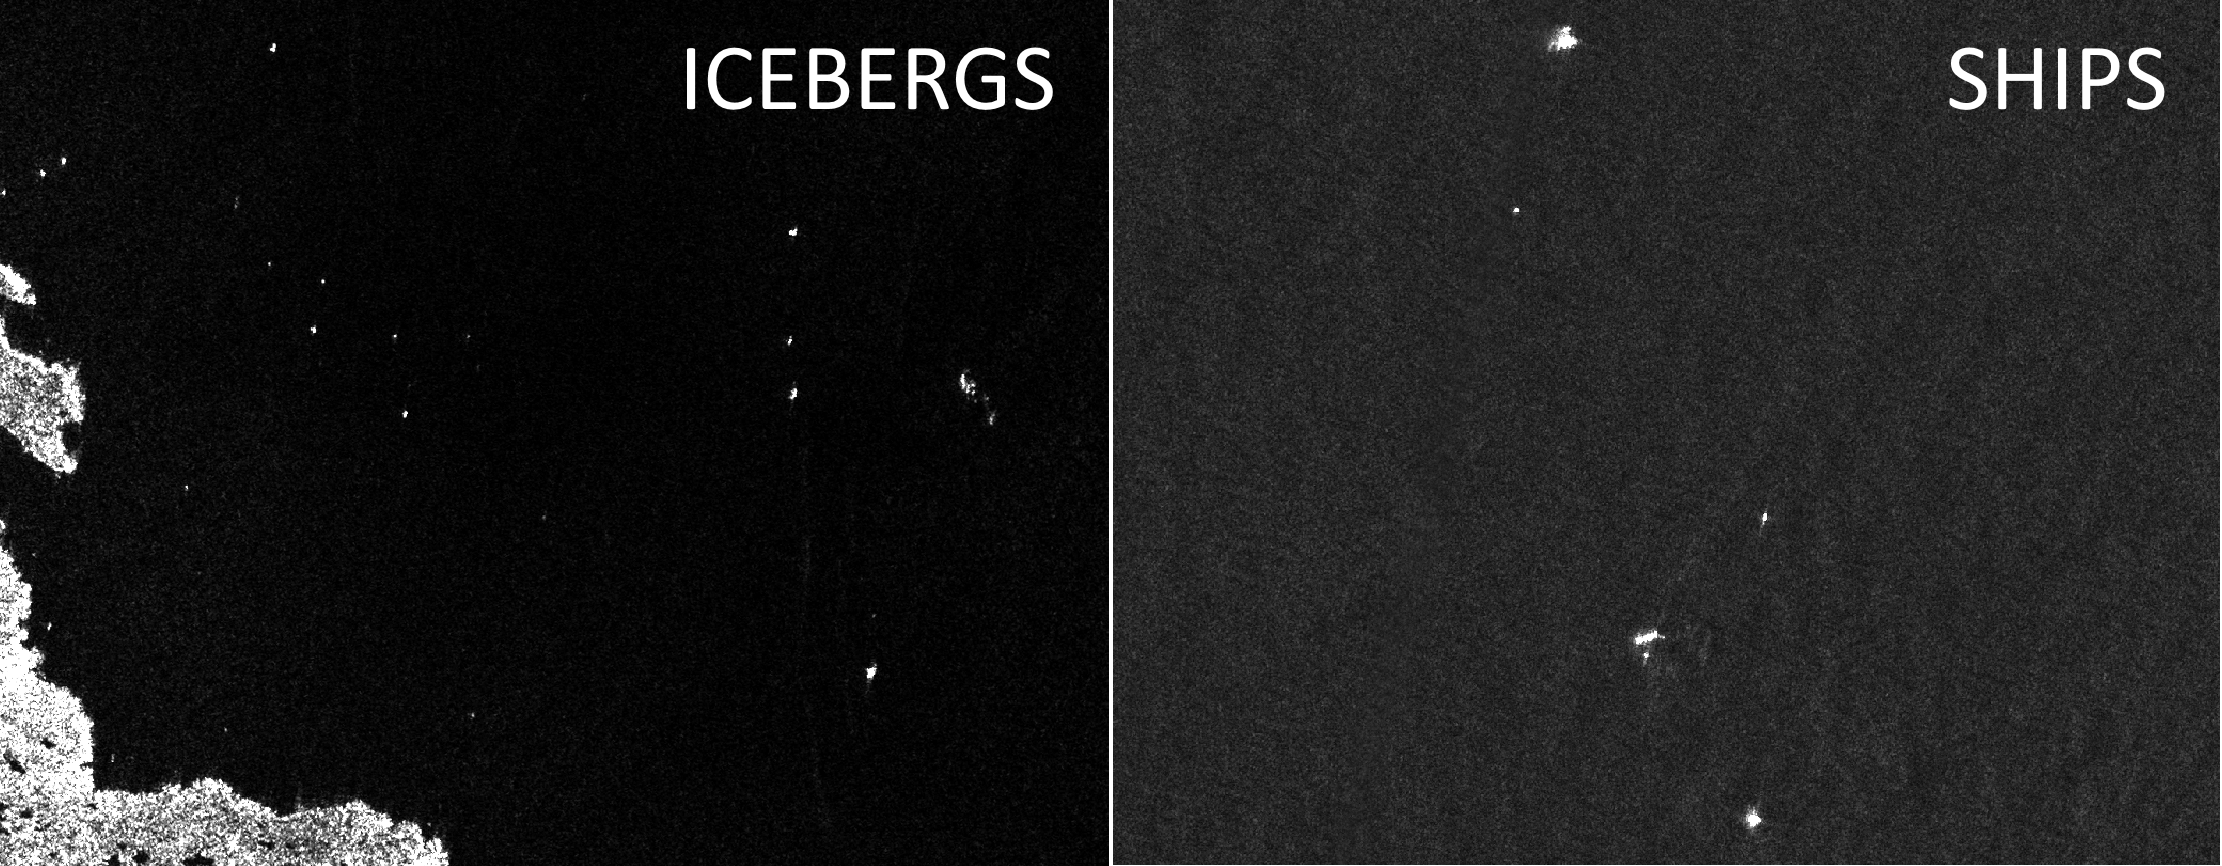
\includegraphics[scale=0.125]{ship-iceberg}

\cite{kaggle}
It is clear from this image why classification is potentially such a problem as it is difficult for a human to classify these images. 

The actual radar images are difficult to visualise because the range of signal strength within a band varies by a factor of $10^{38}$. Therefore, before visualising, the images had to be standardised using z-score. The z-score is calculated in the function below \cite{z-score}:
\begin{lstlisting}{language=python}
def z_score(image_list):
    standardised_image_array = (np.array(image_list) -np.mean(image_list)) / np.std(image_list)
    return standardised_image_array.tolist()
\end{lstlisting}

The images shown below were generated using the following function.
\begin{lstlisting}{language=python}
def plotImage(standardised_list):
    standardised_image = np.array(standardised_list).reshape(75,75)
    plt.imshow(standardised_image)
    return
\end{lstlisting}

The three images below show the band1, band2 and band3 (average of band1/2) for an iceberg image.

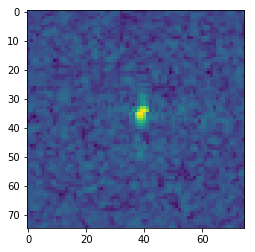
\includegraphics[scale=0.33]{heatmap-iceberg-band-1}
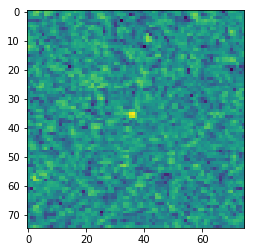
\includegraphics[scale=0.33]{heatmap-iceberg-band-2}
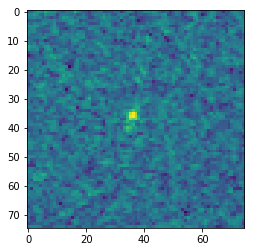
\includegraphics[scale=0.33]{heatmap-iceberg-band3-avg}

The three images below show the band1, band2 and band3 (average of band1/2) for a ship image.

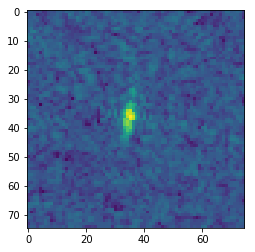
\includegraphics[scale=0.33]{heatmap-ship-band-1}
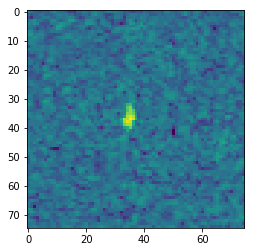
\includegraphics[scale=0.33]{heatmap-ship-band-2}
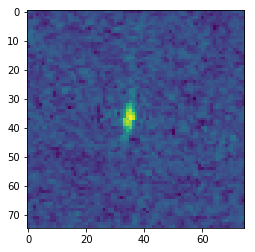
\includegraphics[scale=0.33]{heatmap-ship-band3-avg}

From these images we can see the difference in the output of the different polarisations, we can also see that the resolution means that the object to classify only occupies a small part of the image. The images are also quite noisy as can be seen with the backscattering from the surrounding sea. This further complicates the classification. 

 
\subsection{Algorithms and Techniques}
I will be using a convolutional neural network (CNN) to solve this problem. These have had success in other image classification problems and so I expect them to perform well here. The model will use the pre-trained VGG16 model with weights from imagenet. This is a 16 layer CNN trained on labelled images from the imagenet database. By using the VGG16 pre-trained model to extract features from the images, I have been able to greatly reduce the training time of my own CNN. I had initally hoped to experiment with the ResNet50 and InceptionResNetV2 pretrained models as well. However, these models have a minimum image size of 197x197 and 139x139. As my data is 75x75 images, I could not use them. Instead I used the Xception model, which is also available as a Keras pre-trained model and accepts images of minimum size 71x71 \cite{keras-layers}. 

I have a number of parameters that can be tuned to optimise the CNN:
\begin{itemize}
\item Image data generator - The preprocessing step of creating an image generator has several parameters that can be set. E.g. Horizontal flip, zoom range and rotation range
\item Batch size - How many images should be processed through the CNN at a time
\item Number of epochs - How many times should all the data be run through the network to train it. Increasing this may improve accuracy but adds training time
\item Optimiser - Keras provides different standard optimisers to update weights and alter the learning rate. E.g. Adam, rmsprop, sgd
\item Depth of fully connected layer - The fully connected layer is highly tune-able as I can add or remove layers as required. The effect of this will depend on the layers added. E.g. adding a large dense layer may increase the training time but may also increase the maximum accuracy the model will converge to. 
\item Layer parameters - There are several parameters that can be set for each layer. E.g. Dense layer can set the number of neurons, dropout can set the proportion of neurons to randomly drop
\end{itemize}

\subsection{Benchmark}
At the time of writing the scores on the leaderboard show a top score log loss of 0.0958. To be realistic, I am not expecting my model to outperform this as the leaderboard will constantly improve and there may be several people collaborating in each Kaggle team. A more realistic benchmark would be the median of all the entries which has a log loss of 0.2128 \cite{kaggle}.
The closest benchmark available outside of Kaggle are the results of the German Aerospace Center \cite{bentes} who performed ship-iceberg discrimination using high resolution images from the TerraSAR-X satellite. This achieved recall of 100\% of icebergs with an F1-score of 98\%. However this was using high resolution images on a different satellite so is not an exact equivalent. The lower resolution of the Sentinel-1 images means we can expect this project to have poorer results than the TerraSAR-X benchmark. 

\section{III. Methodology}
\subsection{Data Preprocessing}
The data were in json format, which is easily readable by the Pandas library. 133 of the images did not have an incidence angle. For these I chose to replace their 'na' values with the average incidence angle. This is because the incidence angle should not be the main parameter affecting classificiation of the images, so the additional image data will be more valuable enough for training the data, to justify adding incorrect incidence angles. This processed using the following code:
\begin{lstlisting}{language=python}
avg_angle = np.mean(filter(lambda x: x != 'na' ,training_frame['inc_angle']))
training_frame['inc_angle'] = training_frame['inc_angle'].replace('na',avg_angle)
\end{lstlisting}

Further image preprocessing was done by using an image data generator. An image data generator creates additional images for the training set, by adding altered images to the set. For example, the image generator could take a set of images and rotate every image by 90 degrees clockwise. This would double the training images for the model without including invalid date. They should be used with caution as some alterations invalidate the date, e.g. flipping an image of text would mean the model could incorrectly classify the backwards letters. The imagedatagenerator used in this project is detailed in the Refinement subsection below.

The images had to be organised into a format that is readable by the keras library. This means it has to be organised into a tensor. The following function performed this task:
\begin{lstlisting}{language=python}
def frameToImagesTensor(training_frame):
    # Use z-score to standardise the image data
    standard_frame1 = training_frame['band_1'].apply(z_score)
    standard_frame2 = training_frame['band_2'].apply(z_score)

    band1 = np.asarray(map(lambda band: np.array(band).reshape(75,75),standard_frame1))
    band2 = np.asarray(map(lambda band: np.array(band).reshape(75,75),standard_frame2))
    
    band3 = (band1 + band2)/2
    channel_last_tensor = np.stack((band1,band2,band3),axis=3)
    return channel_last_tensor
\end{lstlisting}
This function output a tensor with the channels last, which is the default method for keras. It also created a third band which was an average of the first two. This colourmap was shown inthe competition description and made identification by sight between an iceberg and a ship easier. Therefore I expect it will assist the neural network as well. 

Finally the data had to be prepared in a way to submit to the model. As the model injects the incidence angle as an input part way through, the generator required special construction to allow the model to read the incidence angle. To solve this problem I used the approach used by one Kaggle kernel that manually created the generator rather than using the keras library, as seen in the following function \cite{angle-inject-kernel}. 
\begin{lstlisting}{language=python}

def gen_flow_for_two_inputs(x,angle_factor,y, batch_size):
    gen = ImageDataGenerator(horizontal_flip = True,
    	vertical_flip = True,
    	zoom_range = 0.2,
    	rotation_range = 360)
    gen_x = gen.flow(x,y,batch_size=batch_size,seed=0)
    gen_angle =  gen.flow(x,angle_factor,batch_size=batch_size, seed=0)
    while True:
        x1i = gen_x.next()
        x2i = gen_angle.next()
        yield [x1i[0], x2i[1]], x1i[1]
\end{lstlisting}
The function creates two generators and then yields the relevant outputs of them. This means the function returns a generator that can be used to input data into the model. 


\subsection{Implementation}
I will be using the keras library with tensorflow-gpu backend to build the CNN. The convolutional layers will be supplied by a transfer model based on weights from imagenet. Additional full connected layers follow this and will combine with the satellite's input angle to form the complete model. The function for creating the CNN using VGG16 as the transfer model is below \cite{angle-inject-kernel}:
\begin{lstlisting}{language=python}
def createCombinedModel():
    angle_input = Input(shape=[1], name="angle_input")
    angle_layer = Dense(1,)(angle_input)
    
    # Use a transfer model for the initial layers
    transfer_model = VGG16(weights='imagenet', include_top=False, input_shape=x_train.shape[1:])
    # Get the output of the last layer of transfer model. Will need to change this for each transfer model
    transfer_output = transfer_model.get_layer('block5_pool').output
    transfer_output = GlobalMaxPooling2D()(transfer_output)
    combined_inputs = concatenate([transfer_output, angle_layer])
    
    combined_model = Dense(512, activation='relu', name="FirstFCDense")(combined_inputs)
    combined_model = Dropout(0.2)(combined_model)
    combined_model = Dense(512, activation='relu', name="SecondFCDense")(combined_model)
    predictions = Dense(1, activation='sigmoid',name="OutputDense")(combined_model)
    
    model = Model(input=[transfer_model.input, angle_input], output =predictions)
    model.compile(optimizer='adam',loss='binary_crossentropy',metrics=['accuracy'])
    return model
\end{lstlisting}
The function above was tuned to reach this configuration, the optimisers were varied and the model structure was changed, as described in the Refinement subsection. The incidence angle is added into the model after the transfer model. This injection of another input meant It was not possible to use a Keras sequential to add layers. Therefore the keras model API was used instead. 
\subsection{Refinement}
See the Algorithms and Techniques section for the list of tune-able parameters. There are a large number of parameters here, too many for me to try all possible combinations. During refinement I chose to vary only a subset of possible parameters. I set the ImageDataGenerator, the batch size and number of epochs for my initial model and found they provided a functional model and therefore did not vary these.  
I have set the image generator to be:

\begin{lstlisting}{language=python}
ImageDataGenerator(horizontal_flip = True,
	vertical_flip = True,
	zoom_range = 0.2,
	rotation_range = 360)
\end{lstlisting}

This allows for horizontal and vertical flips, because icebergs and ships will not look significantly different if their image is flipped. Zoom range of 0.2 as the size will be an important feature by small size changes are unimportant. Rotation range is 360 degrees as the images should be classified the same way, no matter their rotation. 

Batch size = 32 - this allowed for reasonable performance without preventing learning. 
Number of epochs = 100 - this was reached after some initial models took nearly 100 epochs to converge to their best accuracy.

The optimiser did require some tuning. I initially used the RMSprop optimiser as I had used it for previous image classifcation problems. It is also capable of reducing the learning rate over time, but improves upon the Adagrad algorithm by considering only a subset of previous gradients \cite{ruder2016overview}. However, the RMSprop optmiser did not allow the algorithm to converge. I then tried using sgd as it was an algorithm I was more familiar with. I tried tuning the SGD by changing the momentum and setting nesterov to true, however teh model still did not converge. Finally, I used Adam. There is scope for future work to tune the Adam settings or try other optimisers with non-default tuning, however that was beyond the scope of this project. Adam is an advanced algorithm, capable of making use of momentum and adjusting the learning rate of the model overtime. \cite{ruder2016overview}

The depth of the fully connected layer was varied between 1 and 3 layers deep. The first model was a single Dense layer. This achieved a maximum accuracy of 0.53, which is no better than identifying every image as a ship. I increased the neurons  512 and the model did converge and achieved an accuracy of 0.82

The final structure chosen was a Dense layer, a dropout layer and another dense layer. The addition of more dense layers improved the accuracy and the dropout layer should help to prevent overfitting. Initially I used two dense layers of 256 neurons, but the model did not converge and achieved a maximum accuracy of 0.53. Again I increased the neurons per dense layer to 512 and the model did converge and achieved an accuracy of 86\%. This was sufficiently high for me to begin the second stage of the project, which was to vary the transfer learning model. 

\section{IV. Results}
\subsection{Model Evaluation and Validation}
The final model was chosen after experimenting with different optimisers, fully connected layer depths and widths. The final assessment was made by comparing the performance of the Xception transfer model and the VGG16 model. The VGG16 achieved a 3-cross validated accuracy of 86\%. The Xception model reached a 3-fold cross validated accuracy of 88\% and a log loss of 0.246. I have therefore chosen the Xception model as the preferred model for this problem.
	
	
The model was trained using data that had perturbations added by the image data generator. This should ensure the model is able to handle changes to the data. The model is not expected to perform classification beyond sentinel-1 satellite data and therefore is not required to be very robust to new data sources. However, the model could be adapted to handle data from the TerraSAR-x satellites if some alterations were made to the pre-processing steps to allow classification of larger images. Use of the TerraSAR-x data would also allow for experimentation with other transfer learning models, which may perform better on the higher resolution images. 

\subsection{Justification}
The final model did not perform as well as the benchmark models. The benchmarks achieved log loss scores f 0.0958 and this project's final model achieved 0.246. This was expected as this model was constrained by computing power and training time. With additional time the model may have been able to match the benchmark models, which could afford much longer training times. The model's final result is in the mid-range of entries into the Kaggle competition. It did not quite hit my target of 0.213, however some of the folds did reach this level so it is possible that with further training or tuning the model could reach this without re-design. 
\section{V. Conclusion}
\subsection{Free-Form Visualisation}
The chart below shows the change in accuracy for one of the validation folds. From this we can see the model learning very quickly initially and then it's progressed being slowed. Eventually the model stops training as it's validation accuracy has not improved for 10 consecutive epochs, this is due to the early stopping callback function. The graph shows that the model's training accuracy is greater than it's test accuracy, however the difference is not extreme therefore the model is not suffering from excessive overfitting. There is one point in the training process where the training accuracy remains above 90\% but the test accuracy drops to 53\%. That is an instance of overfitting, however the model corrected itself and resolved the overfitting.

The graph shows that the model was still slowly increasing in accuracy but that the progress was inconsistent. With more training time and with the patience of the early stopping function set higher, the model might have improved further. 

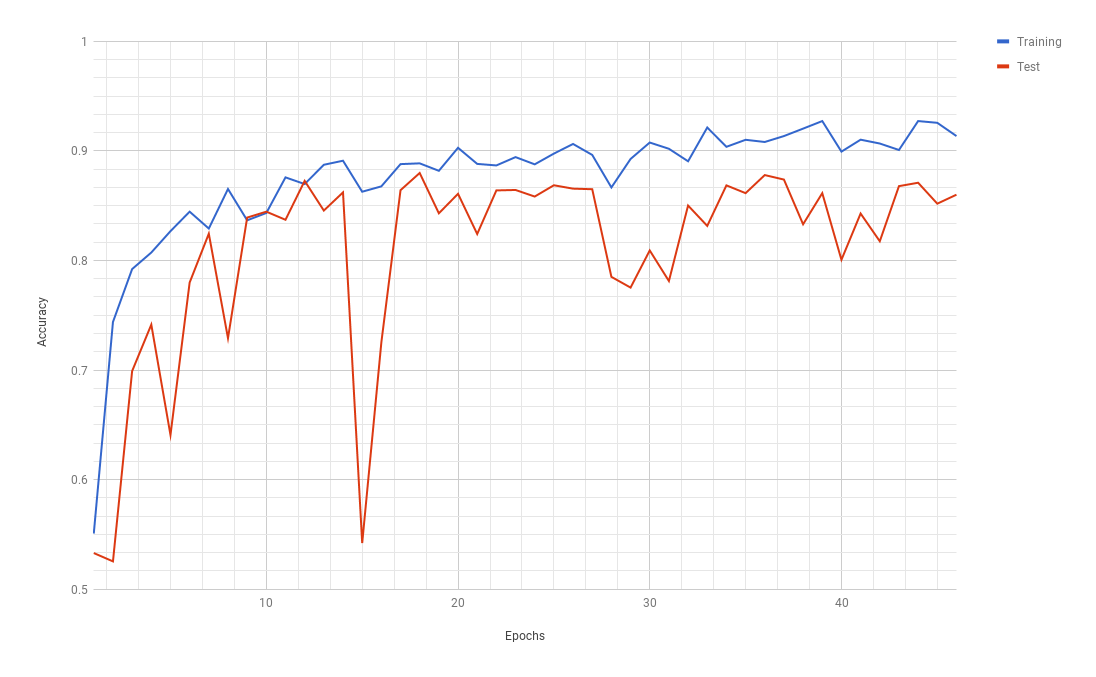
\includegraphics[scale=0.25]{accuracy-chart}

\subsection{Reflection}
I learned a great deal from this project by experimenting with and reading about keras optimisers. Although the final optimiser was using the default settings for the Adam optimiser, I experimented with others and attempted tuning of them. Initially none of my models converged, which was a source of some frustration as it was difficult to identify the root cause. Although this was the hardest part of the project, it was also the one that taught me the most and was therefore the most enjoyable. In future I will be prepared to tune my optimisers and discuss best optimisation strategies. 

Another difficulty of the project was the lack of available information on the data. There was little information about the exact circumstances that images had been taken therefore it was not possible to know the scanning mode used by the satellite to take generate the images. 

The final results are promising but given the problem is one of safety, anything less than 100\% accuracy could result in danger to shipping crews. This project did not achieve the log loss scores of other models and therefore requires more development. The system is accurate enough that it could be valuable if the object being classified was only visible to the satellite. 
\subsection{Improvement}
Currently this model is designed to handle the cross-polarisation data from the sentinel-1 satellites. In order to make use of more data and to generalise the usage of the model, it could be adapted to handle data from other sea-ice monitoring satellites, such as TerraSAR-x or RADARSAT. This would greatly increase the value of the model and would allow it to train on more data, which might improve accuracy. An adaptation of this kind would not be difficult to implement as the only change would be to the pre-processing steps which currently shape the tensor assuming it is as 75x75 image. 

\bibliographystyle{abbrv}
\bibliography{project}{}
\end{document}
